\documentclass{spisok-article}

\title{Среда предметно-ориентированного визуального моделирования REAL.NET}

\author{
	Литвинов Ю.В., доцент кафедры системного программирования СПбГУ,
	y.litvinov@spbu.ru,

	Кузьмина Е.В., студент кафедры системного программирования СПбГУ,
	kuzminaeliz@gmail.com,

	Небогатиков И. Ю., студент кафедры системного программирования СПбГУ,
	ivan.nebogatikov@gmail.com,

	Алымова Д., студент кафедры системного программирования СПбГУ, 
	dalymova96@gmail.com
}

\begin{document}

\maketitle

\begin{abstract}
В статье представлена новая среда для быстрого создания визуальных предметно-ориентированных языков REAL.NET. Эта среда задумывалась как перереализация идей, заложенных в основу системы QReal, с использованием более современных технологий, а также как инструмент и набор библиотек для встраивания средств для работы с визуальными языками в .NET-приложения. В отличие от предшественников, в REAL.NET реализован принцип ``глубокого метамоделирования'', позволяющий рассматривать любую модель как определение языка для другой модели. В этой работе описаны основные принципы, лежащие в основе REAL.NET, её архитектура и возможности, которые реализованы на данный момент.
\end{abstract}

\section{Введение}

Предметно-ориентированное визуальное моделирование активно применяется в целом ряде областей --- в образовательной робототехнике~\cite{portsmore1999robolab}, математических расчётах\footnote{The MathWorks, Inc. Simulink home page. –– URL: \url{http://www.mathworks.com/products/simulink/index.html} (дата обращения: 24.04.2017г)}, создании различного рода программных систем~\cite{luoma2004defining}, при этом наблюдается повышение производительности труда программистов в несколько раз~\cite{kelly2000visual} и существенное снижение ``порога вхождения'', так что писать несложные программы могут даже дети дошкольного возраста (см.~\cite{portsmore1999robolab}). Существует большое количество инструментов, позволяющих быстро создавать новые визуальные языки и инструменты для работы с ними (DSM\footnote{Domain-Specific Modeling, предметно-ориентированное моделирование}-платформы), такие как MetaEdit+~\cite{kelly2008domain}, Eclipse Modeling Project~\cite{gronback2009eclipse}, разрабатываемая студентами и преподавателями кафедры системного программирования СПбГУ среда QReal~\cite{terekhov2013qreal,kuzenkova2013qreal,kuzenkova2011qreal}. Тем не менее, предметно-ориентированные визуальные языки встречаются в индустриальной практике удивительно редко, если учесть преимущества от их применения. Как представляется, это связано с недостатком удобных инструментов и методов для работы с ними.

Если в мире Java-технологий стандартом де-факто для научных и индустриальных применений предметно-ориентированных визуальных языков является Eclipse Modeling Project~\cite{gronback2009eclipse}, то для .NET-приложений существует лишь среда Microsoft Modeling SDK (ранее известная как DSL Tools~\cite{cook2007domain}), которая, хоть и входит в поставку последних версий Microsoft Visual Studio, практически не развивается с 2007 года и в силу особенностей реализации не может быть использована вне Visual Studio. Поскольку проект QReal с развитием и массовым внедрением среды программирования роботов TRIK Studio~\cite{litvinov2015trikstudio}, разрабатываемой на базе QReal, стал слишком неудобен для экспериментов с визуальными языками, было решено начать разработку новой среды, аналога QReal, на платформе .NET, частично с целью получить новую легковесную и простую в модификации платформу для научных применений, частично с целью предоставить .NET-сообществу удобные средства для работы с визуальными языками, которые могут быть встроены в любое .NET-приложение.

В этой статье описаны основные принципы, которые легли в основу REAL.NET, а также некоторые подробности её внутреннего устройства. Эта среда является одной из немногих разработанных ``с нуля'' сред, использующих подход ``глубокого метамоделирования'', поэтому опыт её создания может иметь научное значение как ещё одна апробация этого подхода. Также будут описаны реализованные (или находящиеся в процессе реализации) на данный момент возможности среды, которая в данный момент находится в активной разработке.

\section{Глубокое метамоделирование}

В основе инфраструктуры для задания синтаксических правил визуального языка в REAL.NET лежит принцип ``глубокого метамоделирования''. В распространённых сейчас DSM-платформах (например, всех, упоминавшихся во введении) и в известных стандартах визуальных языков (например, UML, BPMN) применяется двухуровневый подход, при котором визуальный язык задаётся с помощью своей метамодели. Метамодель, как грамматика для текстового языка, описывает множество корректных моделей для визуального языка. Любая модель (например, конкретный бизнес-процесс на BPMN) соответствует своей метамодели (метамодели языка BPML). Метамодель сама часто задаётся в графическом виде, в виде модели на некотором визуальном языке, который называется метаязыком (например, для языка UML в роли метаязыка выступает язык MOF), метаязык, сам являясь визуальным языком, как правило, достаточно выразителен чтобы задать самого себя, поэтому дополнительных языков для задания метаязыка не требуется.

Такой подход, общепринятый на сегодня, подвергался критике ещё с 2001 года~\cite{atkinson2001multilevel} в основном из-за проблем со смыслом понятия ``является экземпляром''. Например, на диаграмме классов UML каждый объект является экземпляром некоторого класса, который тоже должен быть где-то описан в модели, но синтаксис языка про это ничего ``не знает''. Для метамодели UML и класс, и объект являются экземплярами языковых конструкций ``Класс'' и ``Объект'' соответственно, которые абсолютно равноправны и никак формально не связаны. Это приводит, например, к тому, что на диаграмме классов могут существовать объекты, не имеющие своего класса в данной модели, и, что даже хуже, отношения между объектами не связаны никак с отношениями между их классами.

Один из способов решения этой проблемы был предложен в работах~\cite{atkinson2001multilevel, atkinson2003model, atkinson2015defence} и назван ``глубокое метамоделирование''. В этом подходе сущность в модели предлагается рассматривать одновременно и как тип, и как экземпляр некоторого типа (авторами был введён термин ``clabject'', который можно перевести на русский как ``класс-объект''). Классы-объекты могут использоваться в моделях и, одновременно с этим, порождать экземпляры, которые сами являются классами-объектами. В нашем примере с диаграммой классов класс является экземпляром типа ``Класс'', но и сам является типом, экземплярами которого являются объекты (возможно, находящиеся на той же диаграмме). Таким образом, даже по формальным соображениям невозможно создать объект несуществующего класса, и отношения между объектами всегда являются экземплярами отношений между их классами. Получилось красивое решение семантических проблем стандарта UML, предлагавшееся, насколько известно авторам, комитету по стандартизации языка, но так и не включённое в стандарт.

Подход глубокого метамоделирования нашёл, тем не менее, своё применение в предметно-ориентированном моделировании, поскольку оказался очень удобен для встраивания в синтаксис языка семантической информации из предметной области. Существуют DSM-платформы, основанные на этом принципе, такие как Melanee~\cite{atkinson2016melanee}, MetaDepth~\cite{delara2010deep, delara2012domain}, WebDPF~\cite{rabbi2016webdpf}. Тем не менее, ни одна из этих платформ не может быть переиспользована нами напрямую в силу несовместимости технологий --- нашей задачей является создание аналогичных средств для .NET, тогда как Melanee разрабатывается на платформе Eclipse Modeling Project, MetaDepth --- не под Eclipse, но на Java, WebDPF --- браузерная среда.

\section{Архитектура REAL.NET}
В реализации REAL.NET глубокое метамоделирование используется не из соображений семантической чистоты определения метамоделей, а по прагматическим соображениям. При разработке среды TRIK Studio на базе QReal мы столкнулись со сложностями при реализации поддержки подпрограмм. Каждая подпрограмма имела реализацию (задаваемую как отдельная диаграмма) и, возможно, несколько мест вызова, где из основной программы или других подпрограмм вызывалась наша подпрограмма. Проблема оказалась с тем, что узел ``Подпрограмма'' обладал свойствами и обычного узла (поскольку он имелся в палитре и его можно было добавить на диаграмму), и типа узлов (поскольку конкретная подпрограмма, появлявшаяся при первом добавлении узла ``Подпрограмма'' с заданным именем на диаграмму, могла вызываться несколько раз, каждый вызов был ``экземпляром'' вызова конкретной подпрограммы). Кроме того, подпрограммы могли иметь параметры, которые отображались как свойства узла, и даже свой собственный внешний вид, что совсем роднило их с блоками. В QReal была реализована ``пользовательская палитра'' (ещё одна палитра рядом с основной, куда добавлялись блоки вызова подпрограмм при их задании), добавлено в метаязык и поддержано в редакторе отношение ``эксплозия'', связывающее вызов и реализацию подпрограммы, а также сделаны масштабные правки в ядре системы для поддержки ``динамических свойств'' и произвольных картинок для конкретных узлов. Всё это совсем не органично ложилось на используемую в QReal двухуровневую схему задания языка, подпрограммы занимали неочевидное место между моделью и метамоделью, и только с большим трудом были поддержаны.

С помощью глубокого метамоделирования вызов конкретной подпрограммы естественно моделируется как экземпляр подпрограммы, которая сама является экземпляром узла ``Подпрограмма'', поэтому с учётом опыта QReal для REAL.NET был выбран именно этот подход. В REAL.NET была реализована метамодель, которую можно рассматривать как экземпляр самой себя с точки зрения глубокого метамоделирования, репозиторий, где хранится эта метамодель, и два редактора, работающих с этим репозиторием и интерпретирующих его содержимое одновременно и как модель, и как метамодель (то есть все сущности и связи между ними видны на сцене и могут быть отредактированы, одновременно с этим те же сущности видны и в палитре и можно добавлять на сцену их новые экземпляры). В будущем планируется иметь возможность добавлять в репозиторий несколько моделей и указывать в редакторе, какую из них считать моделью, а какую --- метамоделью. Также разрабатывается средство проверки ограничений на модели. Общую структуру системы см. на рисунке~\ref{image:architecture}.

\begin{figure}[ht]
	\centering
	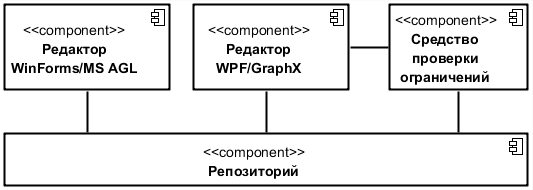
\includegraphics[width=0.8\textwidth]{architecture.png}
	\caption{Общая структура REAL.NET}
	\label{image:architecture}
\end{figure}

При разработке системы активно используются сторонние компоненты. Для хранения моделей в репозитории используется библиотека YC.QuickGraph\footnote{Домашняя страница, URL: \url{https://github.com/YaccConstructor/QuickGraph} (дата обращения: 24.04.2017г.)} (поскольку модели, как выяснилось, не могут быть адекватно выражены в терминах графов, в будущем может потребоваться другое представление). Для разработки редакторов используются две наиболее популярные библиотеки для работы с графами под .NET: GraphX\footnote{Домашняя страница, URL: \url{https://github.com/panthernet/GraphX} (дата обращения: 24.04.2017г.)} и MSAGL\footnote{Библиотека Microsoft Automatic Graph Layout, URL: \url{https://github.com/Microsoft/automatic-graph-layout} (дата обращения: 24.04.2017г)}~\cite{pupyrev2010bundling}. При этом один из редакторов реализован с помощью оконной библиотеки Windows Forms, что делает возможной работу REAL.NET на ОС Linux и Mac OS, второй --- на базе библиотеки WPF\footnote{Windows Presentation Foundation}, что позволяет реализовать более развитый интерфейс под ОС Windows. Наличие одновременно двух редакторов позволяет обеспечить одно из ключевых архитектурных свойств системы --- она не монолит, а набор конфигурируемых и переиспользуемых компонентов. Репозиторий реализован на языке F\#, редакторы и средство проверки ограничений --- на языке C\#.

Далее в статье более подробно описаны основные компоненты системы.

\section{Редактор WPF/GraphX}

Один из прототипов редактора системы REAL.NET реализован с использованием WPF и библиотеки GraphX для платформы .NET, которая позволяет визуализировать графы и поддерживает различные алгоритмы их компоновки. В редакторе использованы такие возможности данной библиотеки как редактирование моделей непосредственно на сцене, а также поддержка различных видов узлов и связей. Для всех типов вершин и ребер, объявленных в репозитории, пользователь может задать нужный вид, после чего у него появляется возможность использовать эти элементы для рисования модели на сцене редактора. Для удобства рядом с элементами модели можно отображать их свойства.

\section{Редактор WinForms/MSAGL}

Microsoft Automatic Graph Layout (MSAGL)~\cite{pupyrev2010bundling} --- это набор библиотечных инструментов для визуализации и редактирования графов, созданный компанией Microsoft. Работа с графом осуществляется через добавленный на форму библиотеки Windows Forms элемент управления. В библиотеке реализованы механизмы автоматического создания визуального представления графа по заданному набору вершин и ребер, функции масштабирования и изменения положения камеры, сохранения отображенного графа в файл, загрузки из файла, функции undo/redo, перемещение вершин и ребер. Самыми большими недостатками MSAGL являются отсутствие документации и регулярных обновлений.

В проекте REAL.NET MSAGL используется для визуального представления и редактирования графа визуального языка программирования. Редактор представляет собой форму библиотеки Windows Forms. Библиотека Windows Forms была выбрана как наиболее кроссплатформенное средство для разработки оконных приложений в .NET.

На данный момент редактор позволяет построить граф по данным, находящимся в репозитории, создавать вершины и ребра в графе и добавлять их в репозиторий. Помимо своего визуального представления каждый узел хранит дополнительную информацию, которую можно посмотреть через редактор с помощью клика мышкой по нужному узлу. Редактор позволяет заменить текущее представление вершины на изображение в формате .png, но эти изменения не сохраняются в репозиторий. Сейчас при любых изменениях графа его визуальное представление перестраивается заново. Исправление этого недочета занимает продолжительное время из-за отсутствия документации по библиотеке MSAGL.

\section{Средства проверки ограничений}

\section{Заключение}

Система REAL.NET находится на данный момент в фазе активной разработки, эта статья не претендует на описание законченного решения. В данный момент не решены такие важные вопросы, как сериализация моделей, выбор модели для отображения в редакторе, интерфейс репозитория для сторонних компонентов. Тем не менее, уже сейчас платформа может использоваться для экспериментов с различными подходами к  метамоделированию, также в ближайшем будущем планируется создание практически полезных визуальных языков на этой платформе. Текущие результаты представлены в GitHub-репозитории проекта~\cite{realNetGithub}.

\renewcommand\refname{Литература}
\begin{thebibliography}{8}
	\bibitem{portsmore1999robolab} M. Portsmore. Robolab: Intuitive robotic programming software to support life long learning //APPLE Learning Technology Review, Spring/Summer. -- 1999.
	\bibitem{luoma2004defining} J. Luoma, S. Kelly, J.-P. Tolvanen. Defining domain-specific modeling languages: Collected experiences //Proceedings of the 4th OOPSLA Workshop on Domain-Specific Modeling (DSM’04) / OOPSLA. –– Jyvävaskylä, Finland : University of Jyvävaskylä, -- 2004.
	\bibitem{kelly2000visual} S. Kelly, J.-P. Tolvanen, Visual domain-specific modeling: Benefits and experiences of using metaCASE tools //International Workshop on Model Engineering, at ECOOP. -- 2000 -- URL: \url{http://dsmforum.org/papers/Visual_domain-specific_modelling.pdf} (дата обращения: 24.04.2017г)
	\bibitem{kelly2008domain} S. Kelly, J.-P. Tolvanen, Domain-specific modeling: enabling full code generation. Hoboken, New Jersey, USA : Wiley-IEEE Computer Society Press, 2008. -- P. 444.
	\bibitem{gronback2009eclipse} R. Gronback. Eclipse Modeling Project: A Domain-Specific Language (DSL) Toolkit. Stoughton, Massachusetts, USA : Addison-Wesley, 2009. -- P. 736.
	\bibitem{terekhov2013qreal} Терехов А.Н., Брыксин Т.А., Литвинов Ю.В. QReal: платформа визуального предметно-ориентированного моделирования. // Программная инженерия, 2013, № 6, С. 11-19
	\bibitem{kuzenkova2013qreal} A. Kuzenkova, A. Deripaska, T. Bryksin, Y. Litvinov, V. Polyakov. QReal DSM Platform: An Environment for Creation of Specific Visual IDEs // Proceedings of 8th International Conference on Evaluation of Novel Approaches to Software Engineering (ENASE 2013), SCITEPRESS, 2013, pp. 251-257.
	\bibitem{kuzenkova2011qreal} Кузенкова А.С., Дерипаска А.О., Таран К.С., Подкопаев А.В., Литвинов Ю.В., Брыксин Т.А., Средства быстрой разработки предметно-ориентированных решений в metaCASE-средстве QReal // Научно-технические ведомости СПбГПУ, Информатика, телекоммуникации, управление. Вып. 4 (128). СПб.: Изд-во Политехнического Университета. 2011, С. 142-145.
	\bibitem{cook2007domain} S. Cook, G. Jones, S. Kent, A.C. Wills. Domain-specific development with Visual Studio DSL Tools. Crawfordsville, Indiana, USA : Addison-Wesley, 2007. –– P. 576.
	\bibitem{litvinov2015trikstudio} Литвинов Ю.В., Кириленко Я.А., TRIK Studio: среда обучения программированию с применением роботов // V Всероссийская конференция <<Современное технологическое обучение: от компьютера к роботу>> (сборник тезисов), СПб., ЗАО <<Полиграфическое предприятие № 3>>, 2015, С. 5-7.
	\bibitem{atkinson2001multilevel} C. Atkinson, T. Kühne, The essence of multilevel metamodeling //International Conference on the Unified Modeling Language. -- Springer Berlin Heidelberg, 2001. -- С. 19-33.
	\bibitem{atkinson2003model} C. Atkinson, Th. Kuhne. Model-driven development: a metamodeling foundation // Software, IEEE. –– 2003. –– Vol. 20, no. 5. –– P. 36–41.
	\bibitem{atkinson2015defence} C. Atkinson, T. Kühne, In defence of deep modelling //Information and Software Technology. -- 2015. -- Т. 64. -- С. 36-51.
	\bibitem{atkinson2016melanee} C. Atkinson, R. Gerbig. Flexible Deep Modeling with Melanee //Modellierung (Workshops). -- 2016. -- Т. 255. -- С. 117-122.
	\bibitem{delara2010deep} J. de Lara, E. Guerra. Deep meta-modelling with metadepth //International Conference on Modelling Techniques and Tools for Computer Performance Evaluation. -- Springer Berlin Heidelberg, 2010. -- С. 1-20.
	\bibitem{delara2012domain} J. de Lara, E. Guerra. Domain-specific textual meta-modelling languages for model driven engineering //European Conference on Modelling Foundations and Applications. -- Springer Berlin Heidelberg, 2012. -- С. 259-274.
	\bibitem{rabbi2016webdpf} Rabbi F. et al. Diagrammatic Development of Domain Specific Modelling Languages with WebDPF //International Journal of Information System Modeling and Design (IJISMD). -- 2016. -- Т. 7. -- №. 3. -- С. 93-114.
	\bibitem{pupyrev2010bundling} L. Nachmanson, S. Pupyrev, M. Kaufmann. Improving layered graph layouts with edge bundling //Proc. 18th Intl. Symp. Graph Drawing (GD’10). -- 2010.
	\bibitem{realNetGithub} Домашняя страница REAL.NET, URL: \url{https://github.com/yurii-litvinov/REAL.NET} (дата обращения: 24.04.2017г).
\end{thebibliography}

\end{document}
